\subchapter{Board setup}{Objective: setup communication
with the board and configure the bootloader.}

After this lab, you will be able to:
\begin{itemize}
\item Access the board through its serial line.
\item Configure the U-boot bootloader and a tftp server
      on your workstation to download files through tftp.
\end{itemize}

\section{Getting familiar with the board}

\begin{center}
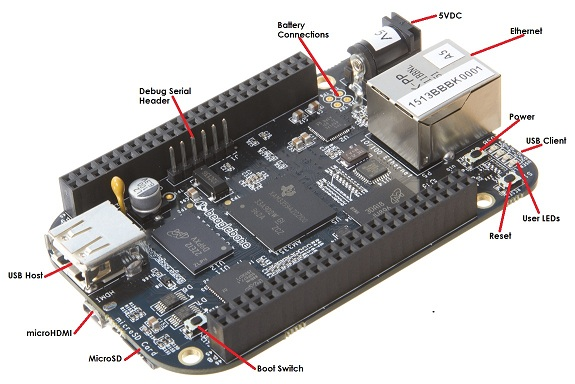
\includegraphics[width=8cm]{labs/kernel-board-setup/beaglebone-black-connectors.jpg}
\end{center}

Take some time to read about the board features and connectors on
\url{http://www.elinux.org/Beagleboard:BeagleBoneBlack}
above image was taken from this page.

Don't hesitate to share your questions with the instructor.

\section{Download technical documentation}

We are going to download documents which we will need during our
practical labs.

The first document to download is the board System Reference Manual found at
\url{https://github.com/CircuitCo/BeagleBone-Black/blob/master/BBB_SRM.pdf?raw=true}
\footnote{There is a link to this manual on the above page}.
This is the ultimate reference about the board, giving all the details
about the design of the board and the components which were chosen.
You don't have to start reading this document now but you will need it
during the practical labs.

The second document to download is the datasheet for the
TI AM335x SoCs, available on
\url{http://www.ti.com/lit/ds/symlink/am3359.pdf}. This document will
give us details about pin assignments.

Last but not least, download the Technical Reference Manual (TRM) for
the TI AM3359 SoC, available on \url{http://www.ti.com/product/am3359}.
This document is more than 4700 pages big (20 MB)! You will need it
too during the practical labs.

\section{Setting up serial communication with the board}

The Beaglebone serial connector is exported on the 6 pins close to one
of the 48 pins headers. Using your special USB to Serial adaptor provided
by your instructor, connect the ground wire (blue) to the pin closest
to the power supply connector (let's call it pin 1), and the \code{TX} (red)
and \code{RX} (green) wires to the pins 4 (board \code{RX}) and
5 (board \code{TX}). \footnote{See
\url{https://www.olimex.com/Products/Components/Cables/USB-Serial-Cable/USB-Serial-Cable-F/}
for details about the USB to Serial adaptor that we are using.}

You always should make sure that you connect the \code{TX} pin of the cable
to the \code{RX} pin of the board, and vice versa, whatever the board and
cables that you use.

\begin{center}
\includegraphics[width=8cm]{labs/kernel-board-setup/beaglebone-black-serial-connection.jpg}
\end{center}

Once the USB to Serial connector is plugged in, a new serial port
should appear: \code{/dev/ttyUSB0}.  You can also see this device
appear by looking at the output of \code{dmesg}.

To communicate with the board through the serial port, install a
serial communication program, such as \code{picocom}:

\begin{verbatim}
sudo apt-get install picocom
\end{verbatim}

If you run \code{ls -l /dev/ttyUSB0}, you can also see that only
\code{root} and users belonging to the \code{dialout} group have
read and write access to this file. Therefore, you need to add your user
to the \code{dialout} group:

\begin{verbatim}
sudo adduser $USER dialout
\end{verbatim}

You now need to log out and log in again to make the new group
visible everywhere.

Now, you can run \code{picocom -b 115200 /dev/ttyUSB0}, to start serial
communication on \code{/dev/ttyUSB0}, with a baudrate of \code{115200}. If
you wish to exit \code{picocom}, press \code{[Ctrl][a]} followed by
\code{[Ctrl][x]}.

There should be nothing on the serial line so far, as the board is not
powered up yet.

It is now time to power up your board by plugging in the mini-USB
cable supplied by your instructor (with your PC or a USB power supply at the
other end of the cable).

See what messages you get on the serial line. You should see U-boot
start on the serial line.

\section{Bootloader interaction}

Reset your board. Press a key in the \code{picocom} terminal to stop the U-boot
countdown. You should then see the U-Boot prompt:
\begin{verbatim}
U-Boot>
\end{verbatim}

You can now use U-Boot. Run the \code{help} command to see the available
commands.

Using the \code{version} command, make sure that you have at least version
\code{2013.10}.
\footnote{This will be needed to use the \code{saveenv} command to
save your U-Boot environment settings to the boards' eMMC storage.
Some earlier versions do not support this.}

If you are doing these labs on your own (i.e. without participating to a Free Electrons
course), we ask you to install the U-Boot binary that we compiled and
tested. See the \code{$HOME/linux-kernel-labs/bootloader/beaglebone-black/README.txt}
file for a simple way to do this.

To avoid trouble because of settings applied in previous practical labs,
we advise you to clear the U-Boot environment variables:

\begin{verbatim}
env default -f -a
saveenv
\end{verbatim}

\section{Setting up Ethernet communication}

The next step is to configure U-boot and your workstation to let your
board download files, such as the kernel image and Device Tree Binary
(DTB), using the TFTP protocol through an Ethernet cable.

To start with, install a TFTP server on your development workstation:

\begin{verbatim}
sudo apt-get install tftpd-hpa
\end{verbatim}

With a network cable, connect the Ethernet port of your board to the
one of your computer. If your computer already has a wired connection
to the network, your instructor will provide you with a USB Ethernet
adapter. A new network interface, probably \code{eth1} or \code{eth2},
should appear on your Linux system.

To configure your network interface on the workstation side, click on
the \code{Network Manager} tasklet on your desktop, and select
\code{Edit Connections}.

\begin{center}
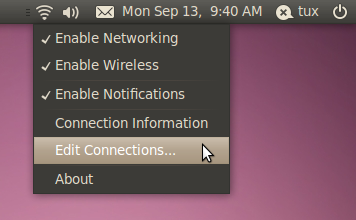
\includegraphics[width=8cm]{labs/kernel-board-setup/network-config-1.png}
\end{center}

Select the new wired network connection:

\begin{center}
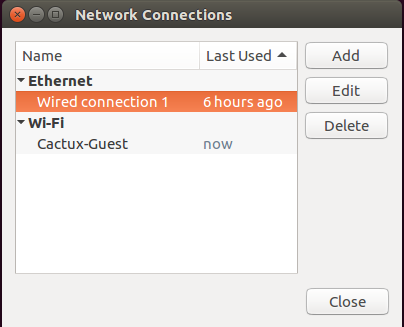
\includegraphics[width=8cm]{labs/kernel-board-setup/network-config-2.png}
\end{center}

In the \code{IPv4 Settings} tab, press the \code{Add} button and
make the interface use a static IP
address, like \code{192.168.0.1} (of course, make sure that this address
belongs to a separate network segment from the one of the main company
network). You will also need to specify the local network mask
(\emph{netmask}, often \code{255.255.255.0}). You can keep the
\code{Gateway} field empty (don't click put the cursor inside the
corresponding text box, otherwise it will ask for a legal value)
or set it to \code{0.0.0.0}:

\begin{center}
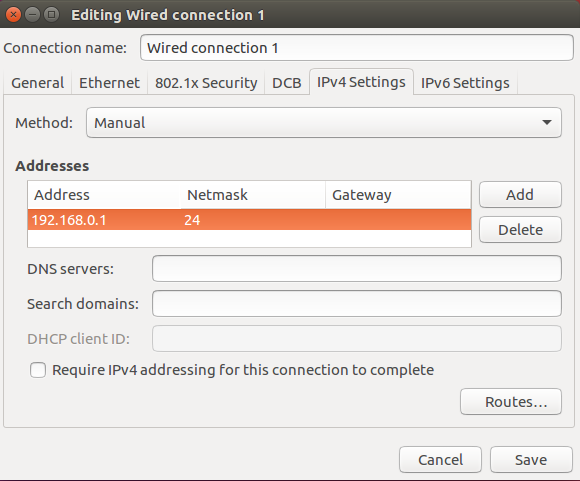
\includegraphics[width=8cm]{labs/kernel-board-setup/network-config-3.png}
\end{center}

Now, it's time to configure networking on U-Boot's side.

Back to the U-Boot command line, set the below environment variables:

\begin{verbatim}
setenv ipaddr 192.168.0.100
setenv serverip 192.168.0.1
\end{verbatim}

Save these settings to the eMMC storage on the board:
\footnote{The U-boot environment settings are stored in some free space
between the master boot record (512 bytes, containing the partition
tables and other stuff), and the beginning of the first partition (often
at \code{32256}). This is why you won't find any related file in the
first partition of the eMMC storage.}

\begin{verbatim}
saveenv
\end{verbatim}

You can then test the TFTP connection.  First, put a small text
file in \code{/var/lib/tftpboot}. Then, from U-Boot, do:

\begin{verbatim}
tftp 0x81000000 textfile.txt
\end{verbatim}

{\bf Caution: known issue in Ubuntu 12.04 and later}: if this command
doesn't work, you may have to stop the server and start it
again every time you boot your workstation:

\begin{verbatim}
sudo service tftpd-hpa restart
\end{verbatim}

The \code{tftp} command should have downloaded the
\code{textfile.txt} file from your development workstation into the
board's memory at location \code{0x81000000} (this location is part of
the board DRAM). You can verify that the download was successful by
dumping the contents of the memory:

\begin{verbatim}
md 0x81000000
\end{verbatim}

We are now ready to load and boot a Linux kernel!
